	\begin{center}
		\section{基础算法}
	\end{center}

	\begin{multicols*}{2}

		\subsection{二维前缀和}

		二维前缀和递推公式。

		\begin{minted}{cpp}
Sum[i][j]=Sum[i-1][j]+Sum[i][j-1]+(G[i][j]=='g')-Sum[i-1][j-1];
		\end{minted}

		\begin{minted}{cpp}
ll lans=Sum[xr][yr]+Sum[xl-1][yl-1]-Sum[xl-1][yr]-Sum[xr][yl-1];
		\end{minted}

		或者调用库函数计算二维前缀和。

		\begin{minted}{cpp}
class NumMatrix {
public:
    vector<vll> Sum;
    ll N,M;
    NumMatrix(vector<vector<int>>& matrix) {
        N=SZ(matrix),M=SZ(matrix[0]);
        Sum.assign(N+5,vll(M+5,0));
        FOR(i,0,N-1){
            partial_sum(all(matrix[i]),Sum[i+1].begin()+1);
        }
        FOR(i,2,N){
            FOR(j,1,M){
                Sum[i][j]=Sum[i][j]+Sum[i-1][j];
            }
        }
    }
    int sumRegion(int row1, int col1, int row2, int col2) {
        row2++;col2++;
        ll ans=Sum[row2][col2]+Sum[row1][col1]-Sum[row1][col2]-Sum[row2][col1];
        return ans;
    }
};
		\end{minted}

		\subsection{二维差分}

		\begin{minted}{cpp}
class Solution {
public:
    vector<vector<int>> rangeAddQueries(int n, vector<vector<int>>& queries) {
        vector<vii> diff(n,vii(n));
        FOR(i,0,SZ(queries)-1){
            ll l1=queries[i][0],r1=queries[i][1],l2=queries[i][2],
            r2=queries[i][3];
            diff[l1][r1]+=1;
            if(r2+1<n) diff[l1][r2+1]-=1;
            if(l2+1<n)diff[l2+1][r1]-=1;
            if(l2+1<n && r2+1<n) diff[l2+1][r2+1]+=1;
        }
        FOR(i,0,n-1){
            partial_sum(all(diff[i]),diff[i].begin());
        }
        FOR(i,1,n-1){
            FOR(j,0,n-1){
                diff[i][j]=diff[i][j]+diff[i-1][j];
            }
        }
        return diff;
    }
};
		\end{minted}

		\textbf{原理解释（容斥原理）}：差分矩阵的特性是——对 $D[x][y]$ 加上 $V$ 后，在后续求前缀和还原矩阵时，以 $(x,y)$ 为左上角、直到矩阵右下角的所有元素都会被加上 $V$。所以想让矩形 $[x_1,x_2]\times[y_1,y_2]$ 恰好加 $V$，就是拿四个这样的「右下四分之一平面」互相抵消：

		\begin{enumerate}
			\item $D[x_1][y_1] \mathrel{+}= V$：让目标区域及右下方的所有点都加 $V$。
			\item $D[x_2+1][y_1] \mathrel{-}= V$：把多加的下方区域减掉。
			\item $D[x_1][y_2+1] \mathrel{-}= V$：把多加的右方区域减掉。
			\item $D[x_2+1][y_2+1] \mathrel{+}= V$：右下方区域被减了两次，所以要加回一次来抵消。
		\end{enumerate}

		\begin{center}
			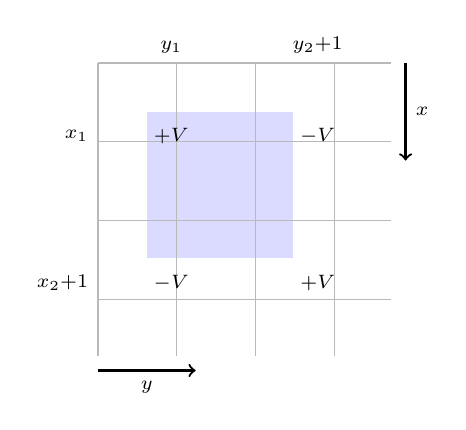
\begin{tikzpicture}[x=0.62cm, y=-0.62cm, font=\scriptsize]
				\fill[blue!14] (1,1) rectangle (4,4);
				\draw[gray!55] (0,0) grid (6,6);
				\node at (1.5,1.5) {$+V$};
				\node at (4.5,1.5) {$-V$};
				\node at (1.5,4.5) {$-V$};
				\node at (4.5,4.5) {$+V$};
				\node[left] at (0,1.5) {$x_1$};
				\node[left] at (0,4.5) {$x_2{+}1$};
				\node[above] at (1.5,0) {$y_1$};
				\node[above] at (4.5,0) {$y_2{+}1$};
				\draw[->, thick] (6.3,0) -- (6.3,2) node[midway, right] {$x$};
				\draw[->, thick] (0,6.3) -- (2,6.3) node[midway, below] {$y$};
			\end{tikzpicture}
		\end{center}

		蓝色是目标矩形，四个格子是打标记的位置：每个标记的作用范围都是「自己往右下无限延伸」，四者叠加后只有蓝色区域净得 $+V$。

		代码里 \texttt{l1,l2} 是行（对应 $x_1,x_2$）、\texttt{r1,r2} 是列（对应 $y_1,y_2$）；四个 \texttt{if} 是越界保护：差分数组没有多开一圈，落在 $n$ 之外的标记本来就影响不到答案，直接丢弃即可。

		\subsection{双指针模板}

		\textbf{参考来源}：\href{https://www.acwing.com/}{AcWing}

		\begin{minted}{cpp}
for (int l = 0, r = 0; r < n; r++) {
    add(a[r]);    // 1 扩展：a[r] 进入窗口
    while (l < r && check(l, r)) l++; // 2 收缩
    // 更新答案    // 3 记录
}
		\end{minted}

		\textbf{三段顺序的硬约束}：

		\begin{enumerate}
			\item 步骤 1 \textbf{必须}在步骤 2 之前——\texttt{check(l, r)} 要用到 \texttt{a[r]} 已在窗口的事实。
			\item 步骤 3 \textbf{必须}在步骤 2 之后——只有收缩到位的 $[l, r]$ 才是当前 $r$ 下的最优左端。
		\end{enumerate}

		AcWing 原始模板把扩展和记录都塞进「具体问题的逻辑」一行注释里，容易让人误以为收缩在记录前面就够了；实际上扩展、收缩、记录三步都不能省、相对位置也不能换。

		\textbf{常见问题分类}：

		\begin{enumerate}
			\item 对于一个序列，用两个指针维护一段区间。
			\item 对于两个序列，维护某种次序，比如归并排序中合并两个有序序列的操作。
		\end{enumerate}

		\subsection{整数二分}

		\begin{minted}{cpp}
bool check(int x) {/* ... */} // 检查x是否满足某种性质

// 区间[l, r]被划分成[l, mid]和[mid + 1, r]时使用：
int bsearch_1(int l, int r)
{
    while (l < r)
    {
        int mid = l + r >> 1;
        if (check(mid)) r = mid;    // check()判断mid是否满足性质
        else l = mid + 1;
    }
    return l;
}
// 区间[l, r]被划分成[l, mid - 1]和[mid, r]时使用：
int bsearch_2(int l, int r)
{
    while (l < r)
    {
        int mid = l + r + 1 >> 1;
        if (check(mid)) l = mid;
        else r = mid - 1;
    }
    return l;
}
		\end{minted}

		也可以用「两端哨兵」写法，核心是先固定不变量：一个端点始终可行，另一个端点始终不可行。这样最后返回哪边不会混。

		\begin{minted}{cpp}
// 最大化答案：check(x) 为 T,T,T,F,F
// invariant: check(lo) == true, check(hi) == false
int lo = L - 1, hi = R + 1;
while (hi - lo > 1) {
    int mid = (lo + hi) / 2;
    if (check(mid)) lo = mid;
    else hi = mid;
}
return lo;

// 最小化答案：check(x) 为 F,F,F,T,T
// invariant: check(lo) == false, check(hi) == true
int lo = L - 1, hi = R + 1;
while (hi - lo > 1) {
    int mid = (lo + hi) / 2;
    if (check(mid)) hi = mid;
    else lo = mid;
}
return hi;
		\end{minted}

		\subsubsection{partition\_point 实现二分答案（C++20）}

		可以知道 \texttt{T,T,T,T,F,F,F,F} 中的第一个 \texttt{F} 出现位置，\texttt{iota} 实现的是这个左闭右开区间，如果想反过来，就是像 \texttt{range2} 一样使用这个 \texttt{reverse} 视图即可。

		\begin{minted}{cpp}
auto check_bs=[&](ll i) {
    return query_is_a_gt_b(i,sec_down_start,memo);
};
auto range1=views::iota(sec_down_start+1,end_of_down);
auto it1=ranges::partition_point(range1,check_bs);
auto range2=views::iota(end_of_down,N+1)|views::reverse;
auto it2=ranges::partition_point(range2,check_bs);

it1=ranges::prev(it1);

ll to_be_select=*it1;
if (it2!=range2.begin()) {
    it2=ranges::prev(it2);
    if (query_is_a_lt_b(*it2,*it1,memo)) {
        to_be_select=*it2;
    }
}
		\end{minted}

		\subsection{三分（实数）}

		凸函数。

		\begin{minted}{cpp}
while(R-L>eps){    // 保证为凸性函数在[l,r]内
    DB mid=L+(R-L)/2;
    if(F(mid-eps)>F(mid+eps)){
        R=mid;
    }else{
        L=mid;
    }
}
		\end{minted}

		还有一种实践方式：使用固定迭代次数代替 \texttt{eps} 阈值。

		\begin{minted}{cpp}
// 方案二：使用固定迭代次数（100次）进行三分搜索。
// 这种方法不依赖eps，更稳定，且100次迭代足以保证精度远高于1e-8。
for(int _=0; _<100; ++_){   // 凹函数，求最小值用的
    DB mid1 = l + (r-l)/3.0; // 推荐用 l + (r-l)/3 的形式，数值上更稳定
    DB mid2 = r - (r-l)/3.0;
    if(fx(mid1) > fx(mid2)){
        l=mid1;
    }else{
        r=mid2;
    }
}
printf("%.11f\n",fx(l));
		\end{minted}

		\subsection{三分整数}

		注意\textbf{整数三分遇到平台都会出现问题}，调整 \texttt{r-l>?} 这个判定阈值也只是缓兵之计，只能保证在小于这个平台的数据上得到正确答案。

		因此正确的想法应该是消除平台（尽可能），比如设计这个 $f$ 函数，\textbf{使其返回值是一个浮点数}，但是仍能反映增减关系（如 $f$ 原来是\textbf{向下取整除法}，可改成\textbf{浮点数除法}）。

		\begin{minted}{cpp}
l=0,r=N-1;
while (r-l>2) {
    ll mid1=l+(r-l)/3;
    ll mid2=r-(r-l)/3;
    if (f(mid1)<=f(mid2)) {
        l=mid1;
    }else {
        r=mid2;
    }
}
FOR(i,l,r) ans=max(ans,f(i));
		\end{minted}

		参考提交：\href{https://atcoder.jp/contests/abc421/submissions/68978595}{AtCoder ABC 421}。

		另一种处理思路：将 $f$ 函数反转（比如加一个符号）使凸函数变为凹函数（相当于沿 X 轴翻折下来），再用普通二分定位极值。

		\begin{minted}{cpp}
ll l=1,r=mn;
while (l<r) {
    ll mid=l+r>>1;
    // if(f(mid)<=f(mid+1)){
    // 从mid点（或其前）开始，函数开始单调递增
    if(f(mid+1)-f(mid)>=0){
        r=mid;
    }else{
        l=mid+1;
    }
}
		\end{minted}

		\subsection{倍增法}

		参考题目：\href{https://www.matiji.net/exam/oj/submit-detail/13507760/29/4498/F16DA07A4D99E21DFFEF46BD18FF68AD}{Matiji 提交记录}。

		首先求出 \texttt{nextPos} 数组（注意：该数组定义是\textbf{结束位置}，所以 \texttt{break} 以后需要 \texttt{-1}），然后从 \texttt{N+1} 开始往前递推。

		\begin{minted}{cpp}
vector<vector<ll> > jump(N+5,vector<ll>(mx_k+2,0));
ROF(i,N+1,1){
    jump[i][0]=i<=N?nextPos[i]+1:N+1;
    FOR(j,1,mx_k){
        jump[i][j]=jump[jump[i][j-1]][j-1];
    }
}
		\end{minted}

		调用方式：

		\begin{minted}{cpp}
FOR(i,1,N){
    ll lans=0,idx=i;
    FOR(j,0,mx_k){
        if(bik[j]){
            idx=jump[idx][j];
        }
    }
    lans=idx-i;
    ans=max(ans,lans);
}
		\end{minted}

		\subsection{LIS 最长上升子序列及其还原}

		\textbf{0-based 输入}，构造时传 \texttt{strict} 开关：\texttt{true} 求严格递增 LIS，\texttt{false} 求单调不降 LNDS（最长非降子序列）。算法核心是 patience sort：严格用 \texttt{lower\_bound} 替换首个 $\geq a_i$，非严格用 \texttt{upper\_bound} 替换首个 $> a_i$。还原阶段反向贪心，严格判 \texttt{<}，非严格判 \texttt{<=}。

		参考提交：\href{https://judge.yosupo.jp/submission/327571}{Yosupo Library Checker}（严格）、\href{https://judge.yosupo.jp/submission/370233}{OpenJudges 单调不降}（长度，非严格还原已通过本地大规模对拍 \(O(N^2)\) 暴力 DP 验证 512/512）。

		\begin{minted}{cpp}
// 最长 (严格 / 非严格) 上升子序列 + 还原值与下标
// 0-based 输入；strict=true → 严格递增, strict=false → 单调不降
struct LIS {
    vector<ll> a;       // 输入序列
    int n;
    bool strict;
    vector<ll> tail;    // patience sort: 长度-i 的子序列最小末值
    vector<int> i_len;  // 以下标 i 结尾的 LIS 长度
    vector<ll> seq;     // 还原的递增子序列值
    vector<int> pos;    // 还原的下标 (0-based, 严格递增)

    LIS(const vector<ll>& v, bool strict_ = true)
        : a(v), n((int)v.size()), strict(strict_), i_len(v.size(), 0) {
        for (int i = 0; i < n; ++i) {
            // 严格 → lower_bound（替换首个 >= a[i]）
            // 非严格 → upper_bound（替换首个 > a[i]）
            auto it = strict
                ? lower_bound(tail.begin(), tail.end(), a[i])
                : upper_bound(tail.begin(), tail.end(), a[i]);
            if (it == tail.end()) {
                tail.push_back(a[i]);
                i_len[i] = (int)tail.size();
            } else {
                int idx = (int)(it - tail.begin());
                tail[idx] = a[i];
                i_len[i] = idx + 1;
            }
        }
        // 反向贪心还原一组解
        int need = (int)tail.size();
        ll cur = LLONG_MAX;
        for (int i = n - 1; i >= 0 && need > 0; --i) {
            bool ok = strict ? (a[i] < cur) : (a[i] <= cur);
            if (ok && i_len[i] >= need) {
                seq.push_back(a[i]);
                pos.push_back(i);
                cur = a[i];
                --need;
            }
        }
        reverse(seq.begin(), seq.end());
        reverse(pos.begin(), pos.end());
    }
    int size() const { return (int)tail.size(); }
};

void Solve(){
    int N; cin >> N;
    vector<ll> P(N);
    for (int i = 0; i < N; ++i) cin >> P[i];
    LIS lis(P);                 // 默认严格；非严格写 LIS lis(P, false);
    cout << lis.size() << "\n";
    for (int p : lis.pos) cout << p << " ";
    cout << "\n";
}
		\end{minted}

		\subsubsection{Dilworth 定理（最小链覆盖 / 偏序划分）}

		偏序集 $(S,\preceq)$ 上，两两\emph{可比}的子集叫\textcolor{blue}{\textbf{链}}，两两\emph{不可比}的子集叫\textcolor{blue}{\textbf{反链}}。

		\textbf{Dilworth 定理}：把 $S$ 划分成链的\emph{最少链数} $=$ \emph{最长反链}的元素个数。\textbf{对偶（Mirsky 定理）}：把 $S$ 划分成反链的\emph{最少反链数} $=$ \emph{最长链}的长度。

		\textbf{落到序列上}（与上面的 \texttt{LIS} 互通），下标先后即时间序：

		\begin{itemize}
			\item 划分成\textbf{最少条不升}子序列 $=$ 最长\textbf{严格上升}子序列长度；
			\item 划分成\textbf{最少条不降}子序列 $=$ 最长\textbf{严格下降}子序列长度；
			\item 对偶：最长\textbf{不降}子序列长度 $=$ 划分成\textbf{最少条严格下降}子序列的数目。
		\end{itemize}

		\textbf{用法}：说白了，从``最少链覆盖''翻到``最长子序列''，只是同时拨两个开关——\textcolor{blue}{\textbf{严格}}$\leftrightarrow$\textcolor{blue}{\textbf{非严格}}、\textcolor{blue}{\textbf{上升}}$\leftrightarrow$\textcolor{blue}{\textbf{下降}}，再套上面那个 \texttt{LIS} 即可。


	\end{multicols*} % 从这里起改用单栏：bigint 是一整个类，行长普遍到 90 列，双栏会被折得满屏折行箭头

		\subsection[\tochl{高精度大整数类}]{高精度大整数类}

		\textbf{什么时候才用它}：答案必须\emph{精确}且超出 \texttt{\_\_int128} 的 $\approx 1.7 \times 10^{38}$。先按这个顺序排除——题目允许取模就取模、$10^{38}$ 以内直接上 \texttt{\_\_int128}（§14.1 有它的读写重载）、只是本地算个常数就用 Python（§18）。都不行，再搬这个类。

		\textbf{实现}：$10^9$ 压位存进 \texttt{vector<int>}（低位在前），零的唯一表示是空 \texttt{vector} 且 \texttt{sign = 1}，\texttt{trim()} 负责维持这个不变量。加减 $O(n)$；乘法先把位宽拆到 $10^6$ 再跑 Karatsuba，$O(n^{\log_2 3}) = O(n^{1.585})$——\textcolor{blue}{\textbf{拆到 $10^6$}} 是因为 Karatsuba 内层是 \texttt{res[i+j] += x[i] * y[j]} 的裸累加，位宽 $10^9$ 时几步就爆 \texttt{long long}；除法是 Knuth 归一化后逐位试商，$O(n(n-m+1))$。符号语义与内建整数完全一致：\textbf{除法向零取整，余数符号跟随被除数}。

		实测（\texttt{-O2}，本机）：$6$ 万位 $\times$ $6$ 万位 $5$ ms，$12$ 万位 $\div$ $6$ 万位 $350$ ms。

		\textbf{六个坑}（本版都已经处理掉，抄的时候别改回去）：

		\begin{itemize}
			\item \texttt{divmod} 的\textbf{除数不能为 $0$}——它上来就读 \texttt{y.a.back()}，除数为零时那是空 \texttt{vector}，直接 UB。调用方自己保证；\texttt{gcd} 内部已经回避了。
			\item \texttt{bigint(int)} 那条构造\textbf{不能删}。字面量 \texttt{0} 同时是空指针常量，少了它，\texttt{b < 0} 会在 \texttt{bigint(long long)} 与 \texttt{bigint(const char *)} 之间二义，直接 CE。
			\item 和 \texttt{long long} 的乘除只在 $|v| \le 9 \times 10^9$ 时走 $O(n)$ 快路径，再大会\emph{自动退化}成大整数乘除——不会算错，但心里要有数。
			\item 输出走 \texttt{str()}，\textbf{不要}改回流传版本的 \texttt{setw + setfill('0')}：那个写法不还原 fill 字符，打完一个大整数之后，同一个流里后面所有 \texttt{setw} 的填充都变成 \texttt{0}。
			\item 流传版本把「乘负数时翻符号」抽成了 \texttt{void check(int v)}，\textbf{传值}——函数里的 \texttt{v = -v} 出不去，于是 \texttt{x *= -3} 静默算错。本版直接写在 \texttt{operator*=} 里。
			\item Karatsuba 合并结果时的进位\textbf{必须是 \texttt{long long}}：\texttt{c[i]} 量级可达 $n \cdot 10^{12}$，一万位往上进位就爆 \texttt{int}。
		\end{itemize}

		随机对拍自测入口：\texttt{template-check/src/\allowbreak bigint\_check.cpp}（与 \texttt{\_\_int128} 逐点比对 $+$ 与竖式乘法比对 $+$ 代数恒等式，改这一节的代码后跑一遍）。

		\begin{minted}{cpp}
// 高精度大整数 bigint：1e9 压位 + Karatsuba 乘法 + 试商长除法
//   加减 O(n)，乘 O(n^1.585)，divmod O(n(n-m+1))，n/m 为压位后的位数（1 位 = 9 个十进制位）
//   语义与 C++ 内建整数一致：除法向零取整，余数符号跟随被除数
//   零的唯一表示是 a 为空且 sign = 1（trim() 维持这个不变量）
struct bigint {
    static constexpr int BASE = 1000000000, W = 9;  // 压 9 位十进制
    // 与小整数运算的 O(n) 快路径上界：a[i] * v 不能爆 long long（9e9 * 1e9 < 9.22e18）
    static constexpr long long SMALL = 9000000000LL;
    vector<int> a;  // 低位在前，每位取值 [0, BASE)
    int sign = 1;   // +1 / -1

    bigint() {}
    bigint(long long v) { *this = v; }
    // 这条 int 重载不能删：字面量 0 同时是空指针常量，
    // 少了它，b < 0 这种写法会在 bigint(long long) 与 bigint(const char*) 之间二义
    bigint(int v) : bigint((long long)v) {}
    bigint(const string &s) { read(s); }
    bigint(const char *s) { read(s); }

    void operator=(long long v) {
        a.clear();
        sign = v < 0 ? -1 : 1;
        // 先转 unsigned 再取反，否则 v = LLONG_MIN 时 -v 溢出（UB）
        unsigned long long u = v < 0 ? -(unsigned long long)v : (unsigned long long)v;
        for (; u; u /= BASE) a.push_back(int(u % BASE));
        if (a.empty()) sign = 1;
    }
    void trim() {  // 去前导零，顺手把 -0 归一成 +0
        while (!a.empty() && a.back() == 0) a.pop_back();
        if (a.empty()) sign = 1;
    }
    bool isZero() const { return a.empty(); }
    bigint abs() const { bigint r = *this; r.sign = 1; return r; }
    bigint operator+() const { return *this; }
    bigint operator-() const { bigint r = *this; if (!r.isZero()) r.sign = -sign; return r; }

    // ---------- 比较 ----------
    static int cmpAbs(const bigint &x, const bigint &y) {  // 只比绝对值
        if (x.a.size() != y.a.size()) return x.a.size() < y.a.size() ? -1 : 1;
        for (int i = int(x.a.size()) - 1; i >= 0; --i)
            if (x.a[i] != y.a[i]) return x.a[i] < y.a[i] ? -1 : 1;
        return 0;
    }
    static int cmp(const bigint &x, const bigint &y) {
        if (x.sign != y.sign) return x.sign < y.sign ? -1 : 1;
        return cmpAbs(x, y) * x.sign;
    }
    // 六个比较运算符。写成 friend 是为了让两侧都能吃隐式转换，
    // b < 0 和 0 < b 都合法（写成成员函数就只有左侧能转）
    friend bool operator<(const bigint &x, const bigint &y) { return cmp(x, y) < 0; }
    friend bool operator>(const bigint &x, const bigint &y) { return cmp(x, y) > 0; }
    friend bool operator<=(const bigint &x, const bigint &y) { return cmp(x, y) <= 0; }
    friend bool operator>=(const bigint &x, const bigint &y) { return cmp(x, y) >= 0; }
    friend bool operator==(const bigint &x, const bigint &y) { return cmp(x, y) == 0; }
    friend bool operator!=(const bigint &x, const bigint &y) { return cmp(x, y) != 0; }

    // ---------- 加减 ----------
    static bigint addAbs(const bigint &x, const bigint &y) {  // |x| + |y|
        bigint r;
        r.a = x.a;
        for (int i = 0, carry = 0; i < int(y.a.size()) || carry; ++i) {
            if (i == int(r.a.size())) r.a.push_back(0);
            r.a[i] += carry + (i < int(y.a.size()) ? y.a[i] : 0);
            carry = r.a[i] >= BASE;
            if (carry) r.a[i] -= BASE;
        }
        return r;
    }
    static bigint subAbs(const bigint &x, const bigint &y) {  // |x| - |y|，要求 |x| >= |y|
        bigint r;
        r.a = x.a;
        for (int i = 0, borrow = 0; i < int(y.a.size()) || borrow; ++i) {
            r.a[i] -= borrow + (i < int(y.a.size()) ? y.a[i] : 0);
            borrow = r.a[i] < 0;
            if (borrow) r.a[i] += BASE;
        }
        r.trim();
        return r;
    }
    friend bigint operator+(const bigint &x, const bigint &y) {
        bigint r;
        if (x.sign == y.sign) r = addAbs(x, y), r.sign = x.sign;
        else if (cmpAbs(x, y) >= 0) r = subAbs(x, y), r.sign = x.sign;
        else r = subAbs(y, x), r.sign = y.sign;
        r.trim();
        return r;
    }
    friend bigint operator-(const bigint &x, const bigint &y) { return x + (-y); }

    // ---------- 与小整数运算（O(n) 快路径，divmod 内部靠它） ----------
    bigint &operator*=(long long v) {
        if (v > SMALL || v < -SMALL) return *this = *this * bigint(v);  // 超出快路径就退化成大整数乘
        if (v < 0) sign = -sign, v = -v;
        long long carry = 0;
        for (int i = 0; i < int(a.size()) || carry; ++i) {
            if (i == int(a.size())) a.push_back(0);
            long long cur = a[i] * v + carry;
            a[i] = int(cur % BASE);
            carry = cur / BASE;
        }
        trim();
        return *this;
    }
    bigint &operator/=(long long v) {  // 向零取整
        if (v > SMALL || v < -SMALL) return *this = *this / bigint(v);
        if (v < 0) sign = -sign, v = -v;
        long long rem = 0;
        for (int i = int(a.size()) - 1; i >= 0; --i) {
            long long cur = a[i] + rem * BASE;
            a[i] = int(cur / v);
            rem = cur % v;
        }
        trim();
        return *this;
    }
    int operator%(int v) const {  // 余数符号跟随被除数；v 取任意 int（含 INT_MIN）
        long long d = v < 0 ? -(long long)v : v, m = 0;
        for (int i = int(a.size()) - 1; i >= 0; --i) m = (a[i] + m * BASE) % d;
        return int(m) * sign;
    }
    friend bigint operator*(bigint x, long long v) { return x *= v; }
    friend bigint operator*(long long v, bigint x) { return x *= v; }
    friend bigint operator/(bigint x, long long v) { return x /= v; }

    // ---------- 大整数乘：拆成 1e6 压位后跑 Karatsuba ----------
    // 拆到 1e6 是为了让 karatsuba 内层 res[i+j] += a[i]*b[j] 累加不爆 long long
    static vector<int> convertBase(const vector<int> &v, int oldW, int newW) {
        vector<long long> p(max(oldW, newW) + 1);
        p[0] = 1;
        for (int i = 1; i < int(p.size()); ++i) p[i] = p[i - 1] * 10;
        vector<int> res;
        long long cur = 0;
        int curW = 0;
        for (int x : v) {
            cur += x * p[curW];
            curW += oldW;
            while (curW >= newW) {
                res.push_back(int(cur % p[newW]));
                cur /= p[newW];
                curW -= newW;
            }
        }
        res.push_back(int(cur));
        while (!res.empty() && res.back() == 0) res.pop_back();
        return res;
    }
    static vector<long long> karatsuba(const vector<long long> &x, const vector<long long> &y) {
        int n = int(x.size());
        vector<long long> res(n + n);
        if (n <= 32) {  // 小规模直接暴力，常数远小于递归
            for (int i = 0; i < n; ++i)
                for (int j = 0; j < n; ++j) res[i + j] += x[i] * y[j];
            return res;
        }
        int k = n >> 1;
        vector<long long> x1(x.begin(), x.begin() + k), x2(x.begin() + k, x.end());
        vector<long long> y1(y.begin(), y.begin() + k), y2(y.begin() + k, y.end());
        vector<long long> x1y1 = karatsuba(x1, y1), x2y2 = karatsuba(x2, y2);
        for (int i = 0; i < k; ++i) x2[i] += x1[i], y2[i] += y1[i];
        vector<long long> r = karatsuba(x2, y2);  // (x1+x2)(y1+y2) - x1y1 - x2y2
        for (int i = 0; i < int(x1y1.size()); ++i) r[i] -= x1y1[i];
        for (int i = 0; i < int(x2y2.size()); ++i) r[i] -= x2y2[i];
        for (int i = 0; i < int(r.size()); ++i) res[i + k] += r[i];
        for (int i = 0; i < int(x1y1.size()); ++i) res[i] += x1y1[i];
        for (int i = 0; i < int(x2y2.size()); ++i) res[i + n] += x2y2[i];
        return res;
    }
    friend bigint operator*(const bigint &x, const bigint &y) {
        vector<int> x6 = convertBase(x.a, W, 6), y6 = convertBase(y.a, W, 6);
        vector<long long> p(x6.begin(), x6.end()), q(y6.begin(), y6.end());
        while (p.size() < q.size()) p.push_back(0);
        while (q.size() < p.size()) q.push_back(0);
        while (p.size() & (p.size() - 1)) p.push_back(0), q.push_back(0);  // 补到 2 的幂
        vector<long long> c = karatsuba(p, q);
        bigint r;
        r.sign = x.sign * y.sign;
        long long carry = 0;  // 必须 long long：c[i] 量级可达 n*1e12，进位早就爆 int
        for (int i = 0; i < int(c.size()); ++i) {
            long long cur = c[i] + carry;
            r.a.push_back(int(cur % 1000000));
            carry = cur / 1000000;
        }
        for (; carry; carry /= 1000000) r.a.push_back(int(carry % 1000000));
        r.a = convertBase(r.a, 6, W);
        r.trim();
        return r;
    }

    // ---------- 大整数除：Knuth 归一化 + 逐位试商 ----------
    // 返回 {商, 余数}；商向零取整，余数符号跟随被除数。除数为 0 是 UB，调用方自己保证
    friend pair<bigint, bigint> divmod(const bigint &x, const bigint &y) {
        int norm = BASE / (y.a.back() + 1);  // 归一化让最高位 >= BASE/2，试商误差 <= 2
        bigint u = x.abs() * norm, v = y.abs() * norm, q, r;
        q.a.assign(u.a.size(), 0);
        for (int i = int(u.a.size()) - 1; i >= 0; --i) {
            // r = r * BASE + u[i]：把被除数的下一位拽下来。
            // 直接在低位插一格是 O(n) 的 memmove，写成 r = r * BASE + u.a[i] 会慢一个数量级
            r.a.insert(r.a.begin(), u.a[i]);
            r.trim();
            int m = int(v.a.size());
            int s1 = int(r.a.size()) <= m ? 0 : r.a[m];
            int s2 = int(r.a.size()) <= m - 1 ? 0 : r.a[m - 1];
            int d = int((1LL * BASE * s1 + s2) / v.a.back());  // 试商，至多偏大 2
            r = r - v * d;
            for (; r < 0; --d) r += v;
            q.a[i] = d;
        }
        q.sign = x.sign * y.sign;
        r.sign = x.sign;
        q.trim();
        r.trim();
        return {q, r / norm};
    }
    friend bigint operator/(const bigint &x, const bigint &y) { return divmod(x, y).first; }
    friend bigint operator%(const bigint &x, const bigint &y) { return divmod(x, y).second; }

    bigint &operator+=(const bigint &v) { return *this = *this + v; }
    bigint &operator-=(const bigint &v) { return *this = *this - v; }
    bigint &operator*=(const bigint &v) { return *this = *this * v; }
    bigint &operator/=(const bigint &v) { return *this = *this / v; }
    bigint &operator%=(const bigint &v) { return *this = *this % v; }

    friend bigint gcd(bigint x, bigint y) {  // 写成迭代，避免大数递归爆栈
        x = x.abs(), y = y.abs();
        while (!y.isZero()) { bigint t = x % y; x = y, y = t; }
        return x;
    }
    friend bigint lcm(const bigint &x, const bigint &y) { return (x / gcd(x, y) * y).abs(); }

    // ---------- 读写 ----------
    void read(const string &s) {
        sign = 1;
        a.clear();
        int pos = 0;
        while (pos < int(s.size()) && (s[pos] == '-' || s[pos] == '+')) {
            if (s[pos] == '-') sign = -sign;
            ++pos;
        }
        for (int i = int(s.size()) - 1; i >= pos; i -= W) {  // 从低位往高位每 W 个十进制位打一包
            int x = 0;
            for (int j = max(pos, i - W + 1); j <= i; ++j) x = x * 10 + (s[j] - '0');
            a.push_back(x);
        }
        trim();
    }
    string str() const {  // 不用 setw/setfill：那会把 cout 的 fill 字符永久改成 '0'
        string s = sign < 0 ? "-" : "";
        s += a.empty() ? "0" : to_string(a.back());
        for (int i = int(a.size()) - 2; i >= 0; --i) {
            string t = to_string(a[i]);
            s += string(W - t.size(), '0') + t;
        }
        return s;
    }
    friend istream &operator>>(istream &is, bigint &v) { string s; is >> s; v.read(s); return is; }
    friend ostream &operator<<(ostream &os, const bigint &v) { return os << v.str(); }
};
		\end{minted}

		用法：

		\begin{minted}{cpp}
void Solve() {
    bigint a, b;
    cin >> a >> b;                 // 支持前导零与正负号
    cout << a + b << "\n";
    cout << a * b << "\n";
    if (!b.isZero()) {
        auto [q, r] = divmod(a, b);  // 一次拿到商和余数
        cout << q << " " << r << "\n";
        cout << gcd(a, b) << " " << lcm(a, b) << "\n";
    }
    bigint f = 1;
    for (int i = 2; i <= 100; ++i) f *= i;
    cout << f.str().size() << "\n";  // 100! 有 158 位
}
		\end{minted}
